\subsection{Methode über die Gravitation}
Das B-Feld wird über die Formel \eqref{eqn:bfeld} bestimmt. $\mu_{0}$ wird dabei als\\
\begin{equation*}
  \mu_{0} = \SI{6.954318602} \cdot 10^{-6} \si{ \frac{N}{A^2}}
\end{equation*}
 angenommen.
In der Anleitung werden die Windungszahl
\begin{equation*}
  N = 195
\end{equation*}
und der Radius
\begin{equation*}
  R = \SI{0.109}{m}
\end{equation*}
der Spule vorgegeben.
Die Stromstärke und das dazu ausgerechnete B-Feld sind in der Tabelle \ref{tab:grav} nachzulesen.\\
$\vec{\mu}_{Dipol}$ wird über die Formel \eqref{eqn:bmom1} berechnet.
Dabei wurde m als
\begin{equation*}
  m = \SI{0.0014}{kg}
\end{equation*}
gemessen und
\begin{equation*}
  g = \SI{9.81}{\frac{m}{s^2}}
\end{equation*}
angenommen.
$\frac{r}{B}$ ist die Steigung der Ausgleichsgeraden der Form
\begin{equation*}
  y = a \cdot x + b.
\end{equation*}
 Die Ausgleichsgrade ist in Abbildung \ref{fig:grav} zu sehen. Die Steigung beträgt
\begin{equation*}
  a=\SI{29.67322 \pm 0.079128}{\frac{m}{T}}.
\end{equation*}
Daraus ergibt sich ein $\vec{\mu}_{Dipol}$ von
\begin{equation*}
  \vec{\mu}_{Dipol} = \SI{0.40753 \pm 0.00109}{A m^2}.
\end{equation*}
\\Der Fehler wird mit Gauß berechnet:
\begin{equation*}
  \Delta \vec{\mu}_{Dipol}= \sqrt{m^2  \cdot g^2 \cdot \Delta a^2}.
\end{equation*}

\newpage
%\documentclass[captions=tableheading]{scrartcl}
%\usepackage{booktabs}
%\usepackage{pdflscape}
%
%
%
%
%\begin{document}
%\begin{landscape}




\begin{table}[h!]
  \centering
  \caption{Gravitation}
  \label{tab:grav}
  \begin{tabular}{c c c  }
    \toprule
     I/A &		B/mT	& r/m	 \\
    \midrule
    1,45 &	1,9663	& 		0,4894\\
    1,6	 &	2,1697	& 		0,8394\\
    1,85 &	2,5088	& 		1,9894\\
    2,1	 &	2,8478	& 	  2,4894\\
    2,1	 &	2,8478	& 	  2,9894\\
    2,2	 &	2,9834	& 		3,4894\\
    2,4	 &	3,2546	& 		3,9894\\
    2,5	 &	3,3902	& 		4,4894\\
    2,5	 &	3,3902	& 		4,9894\\
    2,7	 &	3,6614	& 		5,4894\\
    2,85 &	3,8649	& 		5,9894\\
    2,9	 &	3,9327	& 		6,4894\\
    3,1	 &	4,2039	& 		6,9894\\
    3,3	 &	4,4751	& 		7,4894\\
    \bottomrule
  \end{tabular}
\end{table}

%\end{landscape}
%\end{document}

\newpage
\begin{figure}[h!]
    \centering
    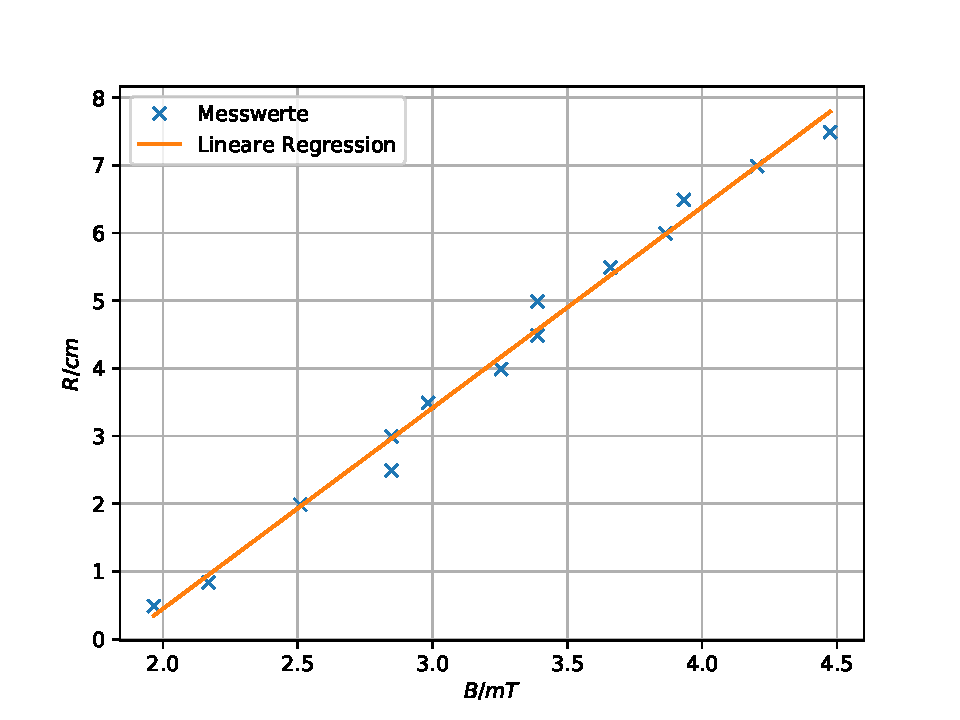
\includegraphics[width=\textwidth]{Gravitation.pdf}
    \caption{Gravitation}
    \label{fig:grav}
  \end{figure}

\subsection{Methode über die Schwingungsdauer}
$\vec{\mu}_{Dipol}$ wird für die Schwingung mit der Formel \eqref{eqn:bmom2} bestimmt.
$J_k$ ist dabei

\begin{equation}
  J_k = \frac{2}{5} \cdot m_k \cdot r^2_k.
\label{eqn:tr}
\end{equation}
\\$m_k$ ist als
\begin{equation*}
  m = \SI{0.124}{kg}
\end{equation*}
\\gemessen worden. $r_k$ beträgt
\begin{equation*}
  r_k = \SI{0.0269}{m}.
\end{equation*}
\\Für $J_k$ ergibt sich daraus ein Trägheitsmoment von
\begin{equation*}
  J_k = \SI{4.11e-5}{kg m^2}.
\end{equation*}
\\Die Steigung der Ausgleichsgeraden zu Tabelle \ref{tab:schwing} in Abbildung \ref{fig:schwing} ist ${T^2B} $  und hat den Wert
\begin{equation*}
  a=\SI{3.91031108 \pm 0.00390843} \cdot 10^{-3} \si{T s^2}.
\end{equation*}
\\In die Formel \eqref{eqn:bmom2} eingesetzt ergibt sich für $\vec{\mu}_{Dipol}$ ein Wert von\\
\begin{equation*}
  \vec{\mu}_{Dipol} = \SI{0.4149457 \pm 0.0000001}{A m^2}
\end{equation*}
Der Fehler wird mit Gauß berechnet:
\begin{equation*}
  \Delta \vec{\mu}_{Dipol}= \sqrt{\frac{(2 \pi)^4 J_{K}^2}{a^4} \cdot \Delta a^2}.
\end{equation*}

%\documentclass[captions=tableheading]{scrartcl}
%\usepackage{booktabs}
%\usepackage{pdflscape}
%
%
%
%
%\begin{document}
%\begin{landscape}




\begin{table}[h!]
  \centering
  \caption{Schwingung}
  \label{tab:schwing}
  \begin{tabular}{c c c c c c }
    \toprule
     I/A &		B/mT	& $\frac{1}{B}/\frac{1}{mT}$ & T/s	& $T^2/s^2$\\
    \midrule
    0,3	& 	0,4068	  & 2,4580	&   3,088 & 	9,5357 \\
    0,5	& 	0,6780		& 1,4748  &   2,438 & 	5,9438 \\
    0,8	& 	1,0849		& 0,9218	&   2,007 & 	4,0280 \\
    1,0 & 	1,3561 		& 0,7374  &   1,784 & 	3,1827 \\
    1,3	& 	1,7629		& 0,5672	&   1,575 & 	2,4806 \\
    1,5	& 	2,0341	  & 0,4916  &   1,431 & 	2,0478 \\
    1,8	& 	2,4410	  & 0,4097  &   1,281 & 	1,6410 \\
    2,0	& 	2,7122 		& 0,3687	&   1,257 & 	1,5800 \\
    2,3	& 	3,1190		& 0,3206	&   1,134 & 	1,2860 \\
    2,5	& 	3,3902		& 0,2950  &   1,09  &   1,1881 \\
    2,8	& 	3,7971		& 0,2634	&   1,044 & 	1,0899 \\
    3,0	& 	4,0683 		& 0,2458  &   0,991 & 	0,9821 \\
    3,5	& 	4,7463		& 0,2107	&   0,943 & 	0,8892 \\
    4,0 & 	5,4244  	& 0,1844	&   0,841 & 	0,7073 \\
    \bottomrule
  \end{tabular}
\end{table}

%\end{landscape}
%\end{document}

\newpage
\begin{figure}[h!]
   \centering
   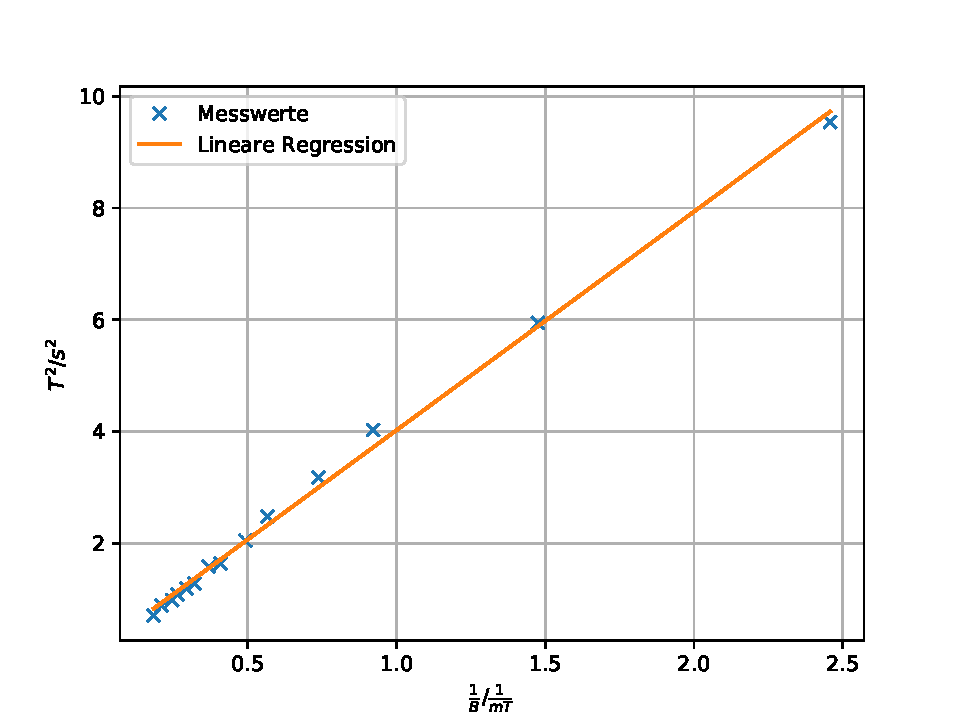
\includegraphics[width=\textwidth]{Schwingung.pdf}
   \caption{Schwingung}
   \label{fig:schwing}
 \end{figure}

\subsection{Methode über die Präzession}
Mit der Formel \eqref{eqn:bmom3} lässt sich $\vec{\mu}_{Dipol}$ für die Präzession bestimmen.
Der Drehimpuls wird berechnet durch \eqref{eqn:lk}. $\nu$ ist hierbei $\nu = \SI{6}{Hz}$.
$J_k$ kann aus dem Aufgabenteil der Schwingung entnommen werden.
\\Für $L_k$ ergibt sich ein Wert von
\begin{equation*}
  L_k = \SI{1.5494e-3}{\frac{kg m}{s}}.
\end{equation*}
Die Steigung der Ausgleichsgeraden zu Tabelle \ref{tab:präzession} in Abbildung \ref{fig:präzession} beträgt\\
\begin{equation*}
 m=\SI{43.67214 \pm 0.00093}{\frac {1}{s T}}.
\end{equation*}
 $\vec{\mu}_{Dipol}$ kann somit auf\\
\begin{equation*}
  \vec{\mu}_{Dipol} = \SI{0.42515559 \pm 0.000000009}{A m^2}
\end{equation*}
 bestimmt werden. Der Fehler wird mit Gauß berechnet.\\
\begin{equation*}
  \Delta \vec{\mu}_{Dipol}=\sqrt{ (2 \pi)^2 {L_K}^2 \cdot \Delta a^2}.
\end{equation*}

\newpage
\input{Präzession.tex}
\begin{figure}[h!]
   \centering
   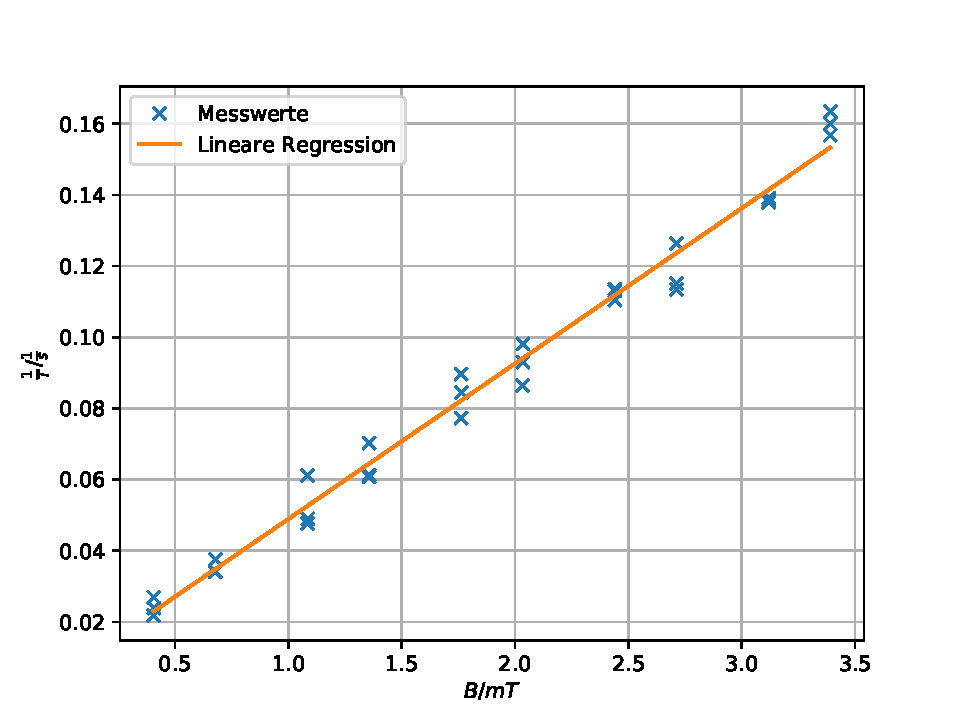
\includegraphics[width=\textwidth]{Präzession.pdf}
   \caption{Präzession}
   \label{fig:präzession}
 \end{figure}
